% This material was originally in Chapter 8 and I really like it. Unfortunately, Microsoft makes filled maps available in Excel 2016 if the user has a 365 subscription. I wrote this section and then discovered that it will not work with every version of Excel 2016. I left it here in case I decide to use it in a future edition or something. 



\subsection{Filled Map}

\begin{center}
	\begin{infobox}{Information}
		\textbf{Filled Maps}
		\\
		\\
		This section concerns creating a 2-D Filled Map in an Excel workbook. These maps are very useful and easy to create, but are only available for Excel $ 2016 $ installations that include a subscription to Excel $ 365 $.
	\end{infobox}
\end{center}


Excel is able to create a map if the data includes any sort of geographical identifiers, like country names, states, counties, or cities. 

\begin{enumerate}
	\item Open workbook \fmtWorksheet{CH8-CancerRate}. This workbook contains the rate of cigarette smoking along with cancer rates for various types of cancer that seem to be related to smoking. The data was captured in a study completed in $ 1960 $.
	\item Click cell \fmtLoc{A3:B43} to activate that range of cells.
	\item Click \fmtButton{Insert $ \Rightarrow $ Charts $ \Rightarrow $ Maps}.
	\item Select \fmtButton{Filled Map}.
	\item Click the map icon.
\end{enumerate}

\begin{figure}[H]
	\centering
	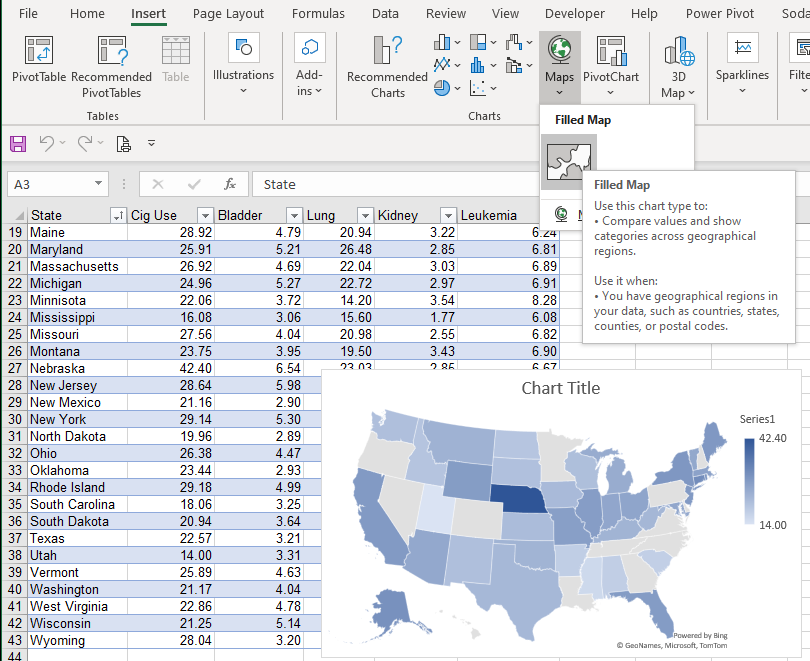
\includegraphics[width=\maxwidth{.95\linewidth}]{gfx/ch08_fig15}
	\caption{Creating a Filled Map}
	\label{08:fig15}
\end{figure}

\begin{enumerate}[resume]	
	\item Excel creates a map of the United States with the cigarette use rate indicated by color. Nebraska has the highest rate of cigarette use and states that are gray, like Oregon, did not have data in the input table.
	\item Click the chart title two times to enable editing. Change that title to \fmtTyping{Cigarette Use}.
	\item Click the paint brush tool at the top right corner of the map to change the style and colors for the map. Click \fmtButton{Color} in the popup menu.
	\item Select \fmtButton{Monochromatic Palette 6}, a green palette.
\end{enumerate}

\begin{figure}[H]
	\centering
	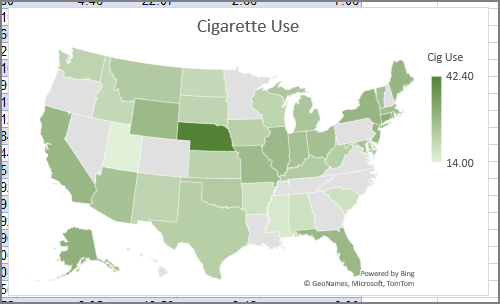
\includegraphics[width=\maxwidth{.95\linewidth}]{gfx/ch08_fig16}
	\caption{Completed Map}
	\label{08:fig16}
\end{figure}

In the same way that the cigarette use rate was mapped, any of the types of cancer can be mapped. The limitation is that only one variable, plus the state names, can be mapped at one time. However, this is a great way for managers to determine, for example, where their customers live so they can plan some sort of promotion.

%%%%%%%%%%%%%%%%%%%%%%%%%%%%%%%%%%%%%%%%%%%%%%%%%%%%%%%%%%%%%%%%%%%%%%%%%%%%

\subsection{Voting Map}

\begin{enumerate}
	\item Open workbook \fmtWorksheet{PR8-Data}.
\end{enumerate}

This workbook includes the percent of Arizona voters who voted for Trump, Clinton, and Other by county in the $ 2016 $ Presidential Election. Mapping this data will help reveal information about the areas of the state the support each of the parties.

\begin{enumerate}[resume]
	\item Click cell \fmtLoc{A3:C18} to activate that range of cells.
	\item Click \fmtButton{Insert $ \Rightarrow $ Charts $ \Rightarrow $ Maps}.
	\item Select \fmtButton{Filled Map}.
	\item Click the map icon.
	\item Once the map is created, change the title to ``Trump Support''.
	\item Double-click the map area, then select the \textit{Data Series} tab (it looks like columns). In the \textit{Series Color} section, select \textit{Red} for the Maximum value and \textit{Orange Accent 2} (a pale orange) for the Minimum value. 
\end{enumerate}

\begin{figure}[H]
	\centering
	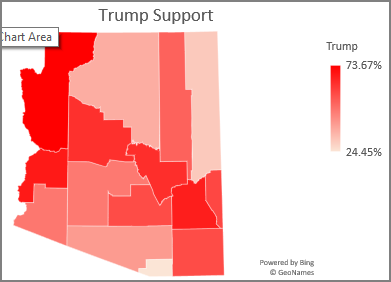
\includegraphics[width=\maxwidth{.95\linewidth}]{gfx/ch08_fig40}
	\caption{The Trump Support Map}
	\label{08:fig40}
\end{figure}

Excel creates a map of Arizona where Trump's percentage is indicated by a red color. The greater his percentage the brighter the color. For example, Mohave County in the top left corner (the northwest part of the state) is bright red because 73.67\% of the voters there supported Trump.

\begin{enumerate}[resume]
	\item Click off of the \textit{Trump Support} map and move it to the top right corner of the worksheet.
	\item Click cell \fmtLoc{A3:B18} and then holding down the \fmtKeystroke{Control} key, click \fmtLoc{D3:D18} to activate those cells.
	\item Click \fmtButton{Insert $ \Rightarrow $ Charts $ \Rightarrow $ Maps}.
	\item Select \fmtButton{Filled Map}.
	\item Click the map icon.
	\item Once the map is created, change the title to ``Clinton Support''.
	\item The default blue color is appropriate for Clinton's map, so that does not need to be changed.
\end{enumerate}

\begin{figure}[H]
	\centering
	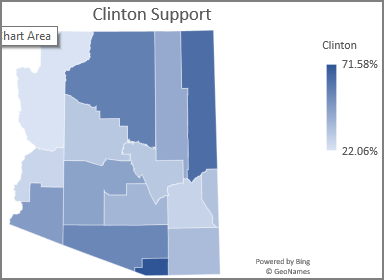
\includegraphics[width=\maxwidth{.95\linewidth}]{gfx/ch08_fig41}
	\caption{The Clinton Support Map}
	\label{08:fig41}
\end{figure}

\begin{enumerate}[resume]
	\item Click off of the \textit{Clinton Support} map and move it to the bottom right corner of the worksheet.
	\item Create a new colum beween \fmtLoc{Column D} and \fmtLoc{Column E}.
	\item Enter \fmtTyping{Delta} in \fmtLoc{E3}.
	\item Click cell \fmtLoc{A3:B18} and then holding down the \fmtKeystroke{Control} key, click \fmtLoc{E3:E18} to activate those cells.
	\item Click \fmtButton{Insert $ \Rightarrow $ Charts $ \Rightarrow $ Maps}.
	\item Select \fmtButton{Filled Map}.
	\item Click the map icon.
	\item Once the map is created, change the title to ``Party Strength''.
	\item Double-click the map area to open the \textit{Format Chart Area} panel.
	\item Click anywhere on the map to open the \textit{Format Data Series} panel.
	\item Open the \textit{Series} tab by clicking the \fmtButton{Columns} icon.
	
\end{enumerate}

\begin{figure}[H]
	\centering
	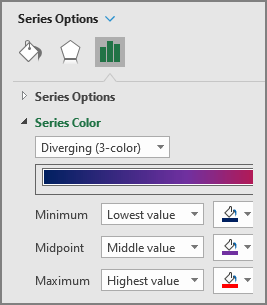
\includegraphics[width=\maxwidth{.50\linewidth}]{gfx/ch08_fig42}
	\caption{Setting The Color Options}
	\label{08:fig42}
\end{figure}

\begin{enumerate}[resume]	
	\item In the \textit{Series Color} section, select \fmtButton{Diverging (3-color)}.
	\item Select blue for the Lowest Value, purple for the Middle Value, and red for the Highest value.
\end{enumerate}

\begin{figure}[H]
	\centering
	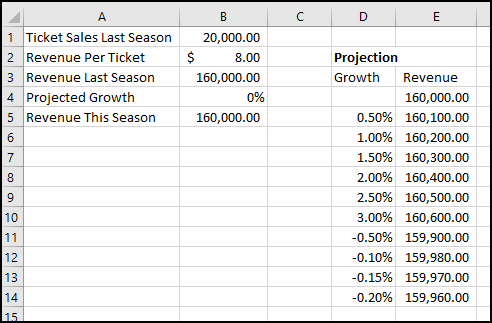
\includegraphics[width=\maxwidth{.95\linewidth}]{gfx/ch08_fig43}
	\caption{The Party Strength Map}
	\label{08:fig43}
\end{figure}

The last map shows the Republican counties in red, the Democratic counties in blue, and the swing counties in purple and indicates the relative strength of each party by county.
